\newpage
\section{Relevant}
 
Una buena representacion de los datos no consiste en presentarlos todos para que el usuario tenga la mayor informacion posible,
consiste en mostrarle los datos necesarios para que pueda hacer una lectura directa de la situacion.\\

En este apartado veremos el refinado de los datos para ofrecer al usuario una informacion relevante y de calidad.

\subsection{Design}
To make a good selection in the dataSet of the fields that are relevant or the combination of these, it is essential to
solid knowledge on the subject to be treated. Therefore, it is fundamental to dedicate the necessary time to enter the
importance of the concept, what benefits it can bring or what situations can dameage us.
The points that should be clear in the design phase are: \\

\textbf{Objective}. Conceptually, what problems do we want to solve or clarify. It is very important that we have a clear objective,
     Even if we do not have prior expertise in the subject, having a well-defined objective helps us find the solution, or
     at least enables us to describe it more clearly to the expert who can solve the problem. \\

\textbf{Important points. Notable situations}. As we mentioned earlier, our goal is not to show all the values, but
     which is about providing the user with important information in order to discover the significant situations that influence the
     us, either positive or negative. At a more technical level, it would be the limits or values of what data are those that provide us with information
     of an exceptional situation, or the values that we are trying to identify more easily. \\

\textbf{Data workflow}. When planning the flow of information, it must be clear how to get from one point to another. For example, 
we should start simple and move to more complex representations.

\subsubsection{How to solve it} 
Once a goal has been set, we must stipulate the necessary fields of the dataSet that we need. That is, we select the fields that interest us. 
Following this, we need to analyze the data provided and see if the list of fields that the source offers us is sufficient to rech the chosen objective.
If not directly, we the combination of them. Next, we decide which values are more outstanding and we will provide them to the user.

\subsubsection{How we solve it. Aire Guru} 
Our main objective is to create awareness of the importance of air pollution in our health. For this we investigate different concepts:
\begin{itemize}
    \item What diseases are affected by air pollution
    \item What pollutans are those that create or influence diseases
    \item What are the sources of each pollutant?
    \item What is the representative measure of the level of air pollution.
    \item How it is calculated and what parameters we need for its calculation
    \item What are the harmful levels in general and for each pollutant
\end{itemize}
The measure that best represents the level of air pollution, in this case is the AQI. The city of Malaga is covered by the European legislation, 
so we focus investigations of official sources in this regulation.
We look for the relationships that pollutants have with different diseases, for this we resort to clinical studies. For each of the diseases, we 
research at the symptoms and how they can be aggravated by each pollutant.
For each pollutant, we look for sources of pollution and see if they occur in the city of Malaga and in what concentrations.
With all this information we define that the pollutants that affect air quality are CO, NO2, O3 and PM (Particulated Material). Dfferent levels of particles
affect different diseases in different ways. \\

As the main objective is awareness, we provide all the data in an organized way in the Glossary of Air Guru. \\

Once these pollutans are selected, we verify if we have the particular data in our dataSet. As we mentioned earlier, some samples show measurements 
from fixed and / or mobile stations and these can be quantitative or qualitative and others can be incomplete. We will have to select the
samples to provide us with the most complete information or the most accurate, in this case the quantitative measure will prevail to the qualitative 
one and in the case that there is only qualitative
the following values are decided: Good: 50, Acceptable: 150, Poor: 300, Bad: 400, Unhealthy: 500 and the user will be informed when the value is qualitative. \\


At this point we know how air pollution affects our health, We make very clear which are the undesirable values by using the alert colors, yellow, orange and 
red. These colors are chosen in the palette of the colors provided by the EAQI.
Height is used in graphics, since it is an intuitive representation for humans. In addition, the icon that represents unhealthy levels of pollution, is
totally different, designed to clearly convey danger. \\
\newpage
\begin{figure}[ht]
    \centering
   \subfigure[BarChart Aire Guru]
    {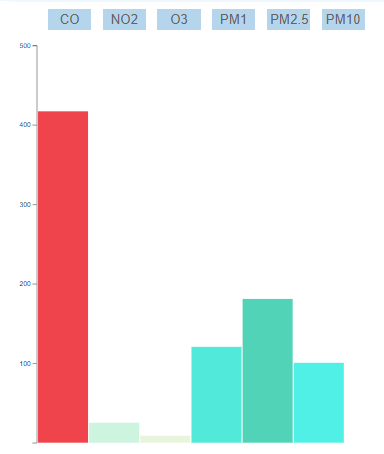
\includegraphics[width=5cm  ]{barchart}}
    \hfill
    \subfigure [Categoria medio ambiente]
       { 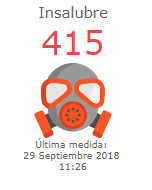
\includegraphics[width=4cm]{unhealthyIcon}}
  
  \caption{Alert situation}
    \end{figure}

    Regarding the workflow, we are guiding the user from the selection of a point in the city of Malaga, either on his own initiative
    or automatic to the details of this point in real time and we continue to show  the evolution of the pollution at that point.
    The logic of this development is that it is anticipated that the user will be interested in the pollution that surrounds him in real time and if
    he wanta to know the breakdown of the pollutants at the point where he is, he can continue to inquire. The map, in addition to showing
    the point where the user is, serves as verification, gives more realism and confidence to the user.

\elsparagraph{Evaluation}  
\begin{itemize}
    \done The objective has been clearly defined and an investigation has been carried out, determining if the dataSet is appropriate.
    \done Worrying levels have been defined as poor, bad and unhealthy and are represented in the Air Guru tool. They stand out clearly so that the user is able to locate them quickly.
     \done The workflow is satisfactory, since the user knows the level of pollution at any location, at a simple glance. It is easy to explore the information further, if the user wishes.
         
\end{itemize}
 

\newpage
\subsection{Credibility and data quality}
It is essential that the credibility of the data set be impeccable. The source of the data must be reliable. In the description of the data, a section must be included where the origin of the data set is explained.

The quality of the data set can be measured according to the following characteristics of the values of the fields: \\
 
\textbf{Precision}. Units of measurement in the correct scale. For example, if we are measuring people's height, it would be meaningless to provide these measurements in meters, since the possible values will be 0, 1 and 2. \\

\textbf{Consistency}. Logical values for each type of field. An example would be a date field, all should
follow the same format. \\

\textbf{Interpretability}. Readable. The data must be clear, both in values and in units. For example, we can not
suppose the unit or scale of the data or, if the data set is dichotomous, "true" or "false", and the values represented are
"A" or "B", we can not assume true = A and false = B without this information being described. \\

\textbf{Complitud}. The data must be consistent in each of the samples. The samples can be differentiated
  from each other, as we see in the Figure below, can share some fields and not others. It would be
better to have a high degree of compliance for the data that interests us in our design.


\begin{figure}[ht]
\centering
\framebox{
\vbox{\begin{tabbing} 
Document \\
\hspace*{5mm} \= Sample 1 \\
\hspace*{10mm}\textit{Field A:} \hspace*{5mm} \= value A \\
\hspace*{10mm}\textit{Field B:} \hspace*{5mm} \= value B \\
\hspace*{5mm} \= Sample 2 \\
\hspace*{10mm}\textit{Field A:} \hspace*{5mm} \= value A \\
\hspace*{10mm}\textit{Field C:} \hspace*{5mm} \= value C \\
\hspace*{10mm}\textit{Field D:} \hspace*{5mm} \= value D \\
\hspace*{5mm} \= ... 
\hspace*{5mm} \= Sample n \\
\hspace*{10mm} \= ... 
\end{tabbing}}%
}
\caption{Example source source document}
\end{figure}

\subsubsection{How to solve it} 
The first step is to compare the information with the source of origin. With the data set and the definition
of each of the fields, the scale and interpretability of the fields and values must be checked.
Then we can perform different analysis of the data to check its consistency and compliance.
It is possible to use different graphs and see if there are extreme or strange values.
Database analysis tools can tell us the completeness of the fields, that is, what percentage of the
samples contain each field.

\subsubsection{How we solve it. Aire Guru} 
The source of data is verified by both the CEMI (Malaga information center) and UrbanClouds, the private company
that collects and sends the data to the city of Malaga.
With the description of the data in the open data portal of Malaga and the information received by UrbanClouds,
we obtain all the necessary information to interpret the data set. \\

For each field, a graphical study has been carried out with the Tableau tool and has verified that the values of the
fields meet the scale and range of expected values, that is, they are precise and consistent.
Using the analysis tools of MongoDBCompas and NoSQLBooster we verify the completeness of the fields needed for our model.
\begin{figure}[ht]
    \centering
    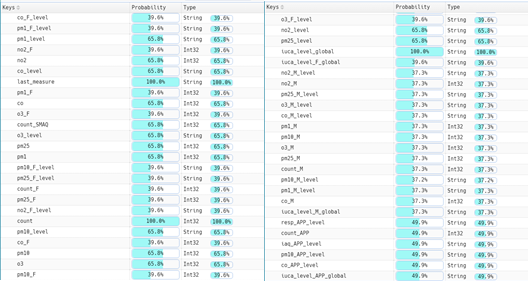
\includegraphics[width=12cm]{noSQLBoosterAnalysis}
    \caption{Completeness analysis}
\end{figure}

\elsparagraph{Evaluation}  
\begin{itemize}
    \done The necessary measures have been taken to verify and understand each of the fields in the data set.
    \done The values of each of the fields have been analyzed by checking scales and ranges.
    \done The completeness of the data has been analyzed.
    
\end{itemize}
 \newpage
\subsection{Enfoque al usuario}
Una gran parte del objetivo marcado en el apartado 3.1 Diseno, viene definido por el servicio que queramos ofrecerle
al usuario, ya que este, es nuestro cliente final y al que pretendermos ayudar.\\


Tendremos que definir las necesidades que muestran los usuarios en combinacion con las carencias del mercado.
Para ello tendremos que decidir si nuestro objetivo esta dirigido a un publico de gran dimension, por lo que tendremos que
que identificar las necesidades homogeneas del usuario medio o si el objetivo esta enfocado a un tipo de usuario
especifico, con necesidades caracteristicas.\\

Por lo tanto necesitamos un estudio actual sobre el nivel psicologico, social y economico del grupo objetivo, para descubrir, no solo
las necesidades, pero tambien los deseos, que le gustaria tener y sus demandas, que quieren.

Una vez los usuarios tengan acceso a los datos tal y como se los proporcionamos, es importante tener una retroalimentacion, 
seria ideal poder realizar un analisis del comportamiento del usuario para ve sus pautas respecto a los datos obtenidos.

\subsubsection{How to solve it} 
Es importante definir a que tipo de usuarios va dirigido. Estudiar tanto sus caracteristicas como la situacion del
mercado.
Utilizar un mecanismo que nos ayude a obtener una retroalimentacion, ya sea por un sistema de puntualizaciones, test o
un mecanismo automatico que permita conocer el comportamiento del usuario. Tambien podremos optar por la combinacion de ambas 
opciones.

\subsubsection{How we solve it. Aire Guru} 
Aire Guru va dirigido a toda la poblacion, por lo que tendremos en cuenta a la hora de implementarlo que la informacion debe
mostrarse de una forma simple, ademas de completa. Ademas, ponemos especial atencion a los usuarios que puedan tener una
enfermedad o condicion medica influenciada por la polucion del aire.
Durante el estudio de mercado, nos dimos cuenta, que muchas de ellas ofrecian la polucion del aire a tiempo real, pero 
pudimos ver las siguientes carencias:
\begin{itemize}
    \item Obsolete measurements. Measurements need to be taken regularly, since there can be huge differences
    between pollution levels at different times of the day.
    \item Limited geographic coverage. The data must cover a reasonable proportion of areas that people spend significant time in.
    \item Insufficiently granular measurements. Measurements must be at a reasonably fine level of granularity. One single measurement for an entire city is not useful.
    \item Poor presentation. Often the information is presented in an uninterpreted form, making it difficult for users to visualize, especially in a geographic sense.
    \item Poor discrimination and interpretation. Many tools show individual values as a number or a colour. This information is not
    enough for the user to take control of their exposure. Such visualizations are not really compelling. 
    \item Exposicion a la polucion de una forma personalizada. Nos interesa saber a que nivel de polucion estamos expuesto
    a lo largo del tiempo, no de forma puntual.
    \item Necesidad de utilizar complicated devices para monitorizar la exposicion. Nuestro objetivo es facilitar la informacion a los 
    usuarios con el minimo de complicaciones posibles.
    \item Sin informacion dedicada por condicion medica. 
\end{itemize}

Una vez implementado, probamos la aplicacion con 14 usuarios. Nuestra herramienta integra Google Analytis que nos permite saber el 
comportamiento de los usuarios, como a cuantas paginas acceden, a cuales y cuanto tiempo permanencen en ella. Ademas, finalizada la prueba,
se realizo una encuesta para medir no solo el nivel de satisfaccion, pero tambien para comprobar la utilidad y si habia conseguido el objetivo.
\begin{figure}[ht]
    \centering
   \subfigure[Aire Guru Form]
    {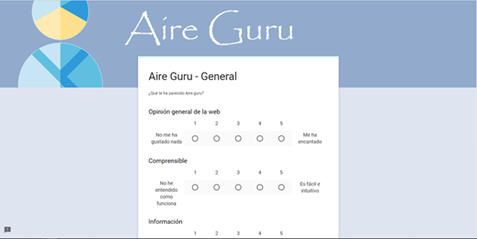
\includegraphics[width=5.5cm  ]{form}}
    \hfill
    \subfigure [Google Analytics]
       { 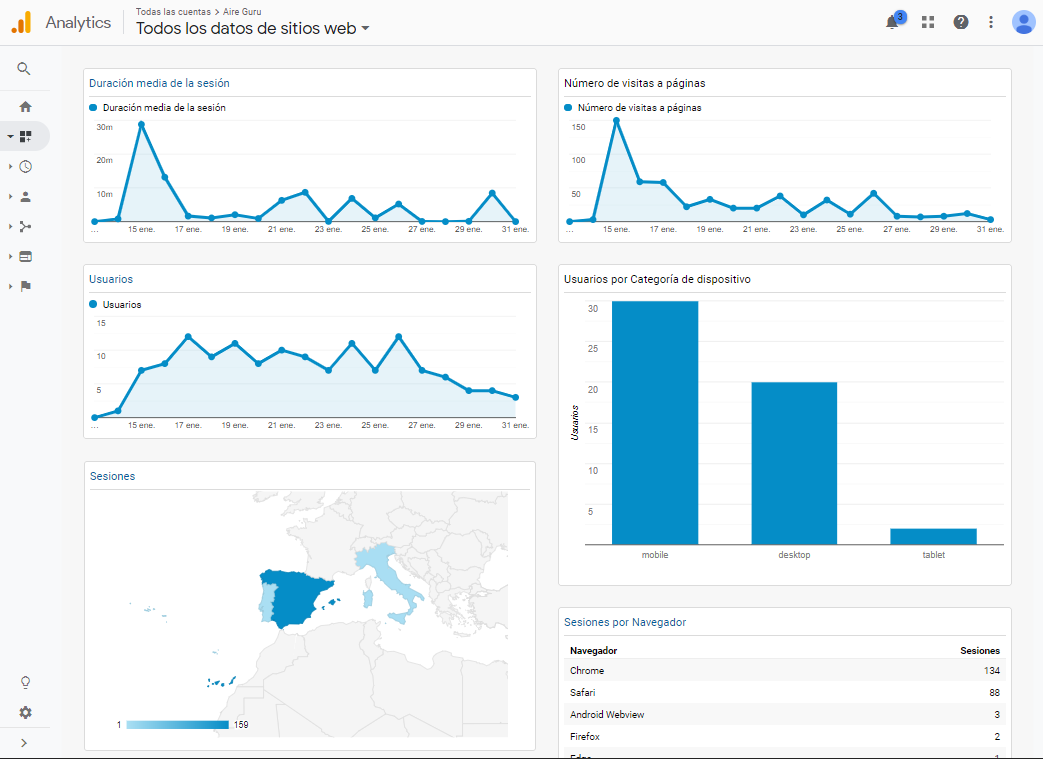
\includegraphics[width=5.5cm]{googleAnalytics}}
  
  \caption{User Feedback}
    \end{figure}
 
\elsparagraph{Evaluation}  
\begin{itemize}
    \done El estudio de mercado nos hizo ver con claridad las carencias que existen en las aplicaciones actuales.
    \done La encuesta nos reporto valoraciones muy positivas respecto a la utilizacion, comprension e informacion reportada.
    \done Usuarios nos comentaron que gracias a Aire Guru habian descubierto que tenian una condicion medica que se puede ver afectada por
    la polucion del aire

\end{itemize}
 

\newpage
\subsection{Util}
Usualmente cometemos el error de intentar mantener al usuario lo mas informado posible y le ofrecemos datos que
no aportan informacion nueva, es redundate.
Debemos centrarnos en que nuestro objetivo no es crear usuarios especializados en la materia, sino aportarles la
informacion de una manera que la puedan aplicar a su vida diaria y asi mejorarla, por lo que huiremos de datos
tecnicos, dificiles de interpretar.

Como mencionamos anteriormente, huiremos de toda aquella informacion vana, que no haga ninguna aportacion
al objetivo marcado. No queremos que el usuario se distraga o se pierda en medio de una piscina de datos completa
pero compleja que para el no tenga ningun sentido. 

Respecto a la representacion, debe seguir el mismo principio, huiremos de decoraciones inecesarias que hagan al 
usuario perderse, solo debe contener la informacion necesaria para poder ser interpretada correctamente, es decir,
toda representacion tienen que contarnos lo que significa sin tener que estar accediendo continuamente a informacion
extra.

En caso complejos, los conceptos que no sean de uso diario para los usuario, podremos poner informacion
complementaria a su disposicion para que el usuario pueda informarse sobre el significado de los datos 
representados, esta practica proporcionara al usuario un mayor dominio del concepto y podra estar mas
seguro de su lectura de los datos, ya que cuando dirigimos al usuario a fuentes oficiales de informacion, donde puedan 
obtener una explicacion veridica,reenforzamos la credibilidad de las representaciones que estamos realizando. En todo caso, 
fuera de la representacion principal, porque el usuario no tendra que acceder a esta informacion continuamente.

\subsubsection{How to solve it} 
Centrarnos en el objetivo, mostrar los datos directamente relacionados con nuestra meta, no annadir los datos 
simplemente porque aparezcan en el conjunto de datos, y no annadir detalles tecnicos irrelevantes para el usuario.


\subsubsection{How we solve it. Aire Guru} 
No util - identificacior de la estacion de medida
 Nos centramos en 6 contaminantes y la medida es unica para todos y el general, el AQI, los rangos son exactamente
 los mismos para todos
 No existen datos que el usuario no entienda, como coordenadas, identificador de la estacion, como se ha tomado la medida.
 Si la medida no existe, simplemente la obviaremos.

\elsparagraph{Evaluation}  
\begin{itemize}
    \done Se ha eliminado la informacion no relevante para el usuario.
    \crossed Se han ofrecido las mediciones exactas. Estos datos son demasiado tecnicos para el usuario. Sin embargo,
    aporta veracidad a los datos y se han  posicionado en un lugar secundario para que no distraiga al usuario.
    
\end{itemize}
 \newpage
\subsection{Personalizacion}
 
    --relevante de manera general vs relevante personal
    --casos personales
    --aplicabilidad
    --solventar problema en particular
    
    
    
    \begin{itemize}
    
          \item Herramientas necesarias para que el usuario entienda la informacion y de porque
     \item conocimientos multidisciplinares
        \item fuentes fiables, actualizacion periodica
    \end{itemize}
  

\subsubsection{How to solve it} 


\subsubsection{How we solve it. Aire Guru} 
 
\elsparagraph{Evaluation}  
\begin{itemize}
    \done
    \crossed
    
\end{itemize}
 \newpage
\begin{figure}[ht]
    \centering
    \framebox{
    \vbox{\begin{tabbing} 
    Check List \\
    \hspace*{10mm} \ding{47} Point 1 \hspace*{25mm} \= \ding{47} Point B \\
     
    \end{tabbing}}%
    
    }
    \end{figure}